\chapter{Is a More Accessible Local Government a More Representative One? The Effects of Online Public Meetings}
\label{chap:dissertation-parts}
    
    
    In response to the growing COVID-19 pandemic, the Denver City Council began hosting their general public meetings online, allowing citizens to attend and participate in discussions virtually. This switch was largely positive for the council, seemingly increasing attendance and active engagement with its meetings. In light of these benefits, and at the request of the public, the council decided to maintain online access to their meetings even after switching back to in-person meetings. Denver was not alone in this continuation of pandemic-era online meetings. Numerous other local governments across the country, citing improved access, still allow citizens to participate or at least watch public meetings virtually.\footnote{Some notable examples include municipal and county governments in Chicago, IL, St. Louis, MO, and Austin, TX} Despite this evidence of success, there has been relatively little work examining the empirical effects these online meetings have on political participation within local governments.

    Public meetings, in particular, are a critical component of American local democracy. They allow citizens to participate directly in the policy-making process \citep{adamsPublicMeetingsDemocratic2004} and act as a conduit through which local officials can learn constituent preferences \citep{einsteinMayorsPartisanshipRedistribution2018,choExperimentingPublicEngagement2021,fungVarietiesParticipationComplex2006}. However, participation in these meetings is rare, and those who attend tend to be socially or economically advantaged compared to their surrounding communities \citep{einsteinWhoParticipatesLocal2019,yoderDoesPropertyOwnership2020}. Scholars and policy advocates have theorized that by reducing participatory costs, online meetings could address these inequities and increase the number and diversity of meeting participants \citep{icmaReflectingVirtualPublic2020}. Yet, in one of the few studies of online meetings \citet{einsteinStillMutedLimited2022} finds that, in the case of planning and zoning meetings, online access fails to engage under-represented groups, and participants are similarly misrepresentative of their surrounding communities. In light of this work, however, we still know relatively little regarding the long-term impacts online meetings had on American local democracy, especially outside the context of the pandemic. Moreover, it remains to be seen how such structural changes to local meetings may have impacted other forms of local governments, such as county councils or school boards.

    Through this article, I examine online meetings' long-term effect on political participation within local public meetings. By leveraging the staggard switch toward and away from online meetings in the years after the pandemic, I estimate the impact online meetings had on the amount and diversity of meeting participants within county, city, and school board governments. Overall, I find that online meetings had mixed effects on local democracy. They increased the average number of public commenters in the aggregate but did not do so universally across types of local government. Some local governments experienced drastic increases in participation following their switch to online meetings, while others experienced no change. While commenters vary significantly between forms of local governments, online commenters were equally misrepresentative of their surrounding community as their offline counterparts. In the rare instance when online meetings alleviated disparities in who participates, other dimensions of inequities, such as race, were exacerbated. Overall, my results suggest that online meetings are potentially an effective tool to expand access to local governments, but in isolation, they are insufficient to address pre-existing inequities in who participates within local democracy.

    \section{Accessibility and Political Participation}
    Attending a local political meeting is a potentially burdensome form of political participation for many individuals. Meetings are often held late into the evening on weekdays in schools or government centers. Individuals likely have to arrange for things such as transportation or childcare to attend. By allowing individuals to participate virtually, online meetings alleviate many of these associated costs, as individuals can watch and participate from anywhere with internet access. Improving political participation by minimizing its social, monetary, or time-related costs is far from a new concept in the study of political science. A broad literature exists documenting the benefits of improved accessibility on political behavior and representation. In the context of elections, vote-by-mail and same-day registration, initiatives can increase turnout, especially among low-propensity voters \citep{barberParticipatoryPartisanImpacts2020,bonicaAllmailVotingColorado2021}. Online access, in particular, can substantially lower the costs of participation as individuals do not have to be physically present to participate. In some instances, digital participation can increase the turnout of traditionally underrepresented groups and attract groups previously disengaged in politics \citep{kruegerAssessingPotentialInternet2002,daltonParticipationGapSocial2017}. Thus, it is reasonable to expect online meetings to have similar long-term effects as they minimize many of the costs associated with commenting at local public meetings. However, evidence exists that increased accessibility does not necessarily translate into positive political outcomes.

    While improvements in political accessibility may make participating easier, they may not foster diverse participation. Without efforts to mobilize under-represented groups in particular, disparities in participation may be reinforced or amplified \citep{verbaVoiceEqualityCivic1995}. Notable examples of this occurring are early voting reforms \citep{burdenElectionLawsMobilization2014}, online political activism \citep{chanPoliticalInequalityDigital2021}, and 311 services \citep{wichowskyCallResponseNeighborhood2022}. In each instance, the reforms designed to make participation more accessible largely reinforced pre-existing socioeconomic divides. Notably, \citet{einsteinStillMutedLimited2022} conclude in their analysis of the early implementation of online meetings that this lack of engagement was one of the critical reasons online meetings failed to diversify public meetings. Thus, online meetings —even in the long term—may be inadequate to improve the diversity of commenters within local meetings unless accompanied by sufficient mobilization and outreach efforts.

    \section{Meeting Participation Across Local Contexts:}

    As required under most state laws, local governments hold meetings open to the public, and most offer an opportunity for citizens to participate directly in the policy-making process. Despite this, previous studies of participation in public meetings have primarily focused on the context of city governments \citep[e.g.,][]{einsteinWhoParticipatesLocal2019}. And they have done this for a good reason. Cities play a prominent role in individuals' lives and are the local government they are most likely to interact with directly. They also tend to offer a plethora of opportunities for input in local policy-making processes \citep{nabatchiDirectPublicEngagement2014a,pinBridgingGapElectoral2022,choExperimentingPublicEngagement2021,wichowskyCallResponseNeighborhood2022} and often rely on these public meetings to gauge public opinion and learn of issues for their constituents \citep{einsteinMayorsPartisanshipRedistribution2018}. In terms of records, cities are also likely to keep high-quality meeting minutes transcripts, which are vital to constructing public meeting participation datasets. However, cities are just some of the local governments to hold public meetings to learn their citizens' preferences and concerns. Both school boards and county governments offer similar opportunities.

    School boards often use public meetings as a vehicle to guide school closures and curriculum changes. Much akin to municipal governments, school boards host various public meetings and forums to inform constituents of upcoming changes or gather community feedback. These meetings and the community connection they provide can be vital for the success of school boards \citep{morelHowCommunityEngagement2021,stoneCivicCapacityUrban2001,tracySpeakingOutPublic2007}, and public policy scholars have paid increased attention to the impact these meetings have both on policy outcomes \citep{morelTakeoverRaceEducation2018,hartneyPoliticsMarketsPandemics2022} and the individuals who participate within them \citep{nuamahCostParticipatingPoor2021,collinsDoesMeetingStyle2021,nuamahCloseHomePlaceBased2021}. While invaluable to our understanding of direct democracy and public education, most studies only examine individual case studies commonly surrounding school closures and rarely examine how the structure/accessibility of the meetings may influence participation \citep[although see][]{collinsDoesMeetingStyle2021}. Understanding whether school boards exhibit the same levels of inequality well-documented at the municipal level is vital, especially as critical issues surrounding race, gender, and public health are increasingly decided at the school board level.\footnote{As an example, see \citet{hartneyPoliticsMarketsPandemics2022}}

    Despite counties' vital role within the American government, they have primarily remained the ``forgotten government" of local politics. We know little about how public participation and opinion shape county-level politics \citep{bentonAssessmentResearchAmerican2005a}. Previous work surrounding counties has primarily examined how the composition and characteristics of public officials have shaped county outcomes \citep[e.g.,][]{mohrStrategicSpendingDoes2019}. Crucially despite the fact that counties are often constrained by both state and municipal governments \citep{petersonCityLimits1981}, they are responsive to constituent preferences and susceptible to traditional political influences \citep{debenedictis-kessnerPoliticsForgottenGovernments2020}. Thus public meeting participation may, as it does at other levels of local government \citep{einsteinWhoParticipatesLocal2019}, play an influential role in county politics. Counties, much like other local governments, hold regular meetings open to the public. Many of these meetings allow the public to comment directly on agenda item issues or other concerns. County governments often use these meetings to gauge the public's support for new budgets, large infrastructure projects, or electoral changes. During the COVID-19 pandemic, these meetings became a vital source of information and expression for citizens surrounded by ever-changing health guidelines and restrictions \citep{lynchPandemicPolitics2022}. We know very little regarding who attends these meetings, the issues they bring up, or the impact of their participation. Do counties experience similar levels of participation found in other local governments, or are they also forgotten in the eyes of their constituents?

    Whether participation in public meetings—or the impacts of improved accessibility—should differ across these local government levels is unclear. In their book examining elections and democracy within local politics, \citet{oliverLocalElectionsPolitics2012} suggest that political participation fundamentally changes as local governments increase in size, scope, and bias.\footnote{As defined by the authors, bias refers to a government's ability to distribute resources among its constituents.} As local governments grow, individuals tend to engage with politics less as their connection to political issues and political efficacy decrease \citep{oliverDemocracySuburbia2001,schlozmanUnheavenlyChorusUnequal2012}. Thus, in the context of public meetings, we should expect differences in participation between school boards, cities, and counties simply due to their differences across these dimensions. In theory, individuals should participate the most in school board meetings, as their ability to enact direct policy change is the greatest and their ties to school board issues the most tangible. Likewise, participation within county governments should be the least due to the wider variety of issues and constituent preferences they must address.

    However, these early conclusions contrast the historically low participation levels across all levels of local government \citep{hopkinsIncreasinglyUnitedStates2018}. Local political issues are often parochial and temporal \citep{oliverLocalElectionsPolitics2012}. The habitual nature and value of repeat participation in national-level politics may not exist in local politics \citep{aldrichTurnoutHabit2011}. While events such as school closings, zoning decisions, or election administration are significant political events for these governments, they likely do not affect individuals on a consistent enough basis to warrant intense engagement \citep[see][]{nuamahCloseHomePlaceBased2021}. Moreover, work such as \citet{hopkinsIncreasinglyUnitedStates2018} or \citet{hershPoliticsPowerHow2020} suggest that individuals care more about national issues and are often disengaged from local political happenings. Therefore, it may not matter how these local governments differ because the American public is equally unengaged across all levels, and participation is dominated by a subset of advantaged individuals \citep[e.g.,][]{einsteinWhoParticipatesLocal2019,yoderDoesPropertyOwnership2020}. Understanding how participation differs between local governments is a critical but unaddressed question in political science. A question this paper hopes to address.

    \section{Public Meeting Data:}
    In order to examine the effects of online meetings and expand coverage beyond previous local boundaries, I construct a novel dataset of public meeting participation from the school board, city, and county governments within St. Louis County, Missouri. I chose St. Louis because of the quality of public records, partly due to Missouri's detailed sunshine law, and the county's many overlapping local governments. By focusing on close or overlapping local governments, I can examine the differential effects online meetings may have while controlling for similar regional, state, or federal factors. All of these are especially important given the surrounding context of the COVID-19 pandemic, which elicited a cooperative response from almost all levels of the American government. In total, I collect records of public participation from 22 school boards, 15 municipal governments, and the county itself. These local governments cover a broad spectrum of sizes, with the largest government being St. Louis County (1,001,982) and the smallest being Brentwood City (8,198). Notably, my sample's city and school board governments are relatively diverse and vary in terms of racial makeup, median income, and home ownership. I provide a more detailed breakdown of my sample's demographics and the selection method used to construct the sample within the Appendix. While far from exhaustive, the novel dataset covers 22\% of the county's municipal populations, 52\% of its school board populations, and the entirety of the county.

    

    For each of these governments, I download and digitize their general meeting minutes from 2018 until late 2022. These are the routine public meetings held by each government. By law, these meetings are open to the public, provide opportunities for public comments, follow a set schedule, and maintain detailed minutes of all topics discussed. Given their routine nature and general purpose, these meetings provide a roughly equivalent comparison point between the three levels of local government within my sample.\footnote{Local governments hold other meetings addressing specific policy issues, such as zoning or industrial development. These meetings are also often open to the public and have been the focus of previous studies of public meeting participation \citep[see][]{einsteinWhoParticipatesLocal2019}.} While each government's meeting minutes vary in terms of how detailed they are, most record the names, addresses, and comments of all individuals who participate in the meeting.\footnote{This includes individuals who submit their comments digitally.} In a few rare instances, local governments only record the total number of commenters present. For these cases, I treat each commenter as a unique individual. I present the detailed breakdown of my final dataset within \autoref{tab:commentSummary}. Overall, my dataset includes over 10,000 unique comments submitted by over 8,000 individuals across approximately 2,213 local political meetings.

    \begin{table}[H] 
        \centering 
        \caption{Summary of Comments Database} 
        \label{tab:commentSummary} 
       \scalebox{1}{
            \begin{tabular}{llcc}
            \\[-1.8ex]\hline 
              \hline \\[-1.8ex] 
            \multicolumn{1}{l}{} & \multicolumn{3}{c}{Level of Government}                              \\ 
            \hline \\[-1.8ex] 
                           & County & City   & School Board     \\
            \hline \\[-1.8ex] 
            Years: & 2018-2022 & 2018-2021 & 2018-2022 \\
            Number of Governments: & 1 & 15 & 22  \\
            Number of Meetings: & $218$ & $1029$ & $966$ \\
            Population Coverage: & $100\%$ & $22\%$ & $52\%$  \\
            First Name: & \ding{51}& \ding{51}& \ding{51}\\
            Last Name:  & \ding{51}& \ding{51}& \ding{51}\\
            Address:  & \ding{51}& \ding{51}& \ding{51}\\
            Number of Comments: & 7069 & 1206 & 1892  \\
            Number of Individuals: & 5621 & 926 & 1555  \\
            Commenting Rate: & 0.56\% & 0.20\% & 0.19\% \\
            \hline\\
            \\[-1.8ex]\hline 
              \hline \\[-1.8ex] 
          \end{tabular}}
          \begin{tablenotes}
              \item {\footnotesize Note:  The table above provides the summary of the universe of comments within the data set. Population coverage refers to the estimated proportion of the population of St. Louis County covered by the sample.}
          \end{tablenotes}
      \end{table}

     
    From this initial dataset, we can gleam some insight into public participation across these levels of government. Participation within these meetings is rare across all three forms of local government.  Only 0.56\% of residents comment at county level meetings over my sample’s four years of coverage, with municipal (0.20\%) and school board (0.19\%) governments experiencing slightly lower rates of participation. Individuals also appear to only comment once within meetings and then disappear from the dataset. In fact across all three levels of local government only 15\% of individuals ever submit more than one comment.\footnote{These low levels of repeat participation are not unique to my dataset. Other datasets of meeting participation such as that from \citet{yoderDoesPropertyOwnership2020} have similarly low levels and cover a far more extensive 10 year timeframe.} On average individuals appear to comment regarding a specific issue and then stop actively participating within local meetings. This pattern falls in line with previous conceptions of local democracy and suggests that participation within this realm is deliberate and motivated \citep{oliverLocalElectionsPolitics2012,nuamahCloseHomePlaceBased2021}. Individuals reach out to their local governments when faced with a pertinent issue and then resume their lives once it has been addressed. In the broader context of this paper, meeting accessibility may be more about encouraging new groups to participate rather than fostering repeat participation. Given the unique overlapping nature of my dataset, I can also examine participation across levels of government.\footnote{To match individuals across levels of local government I fuzzy string match on commenters first and last name. My estimates of cross-level commenting are likely larger than the true rates for my sample.} Are individuals active at one level of local government also active in others? The short answer appears to be no. Cross-level commenting appears exceptionally rare with a little over 1\% of commenters ever commenting at more than one level of local government. While this finding may be a product of the relative short time frame covered by the data, it may provide further evidence of deliberate and conscious participation within local democracy.  Individuals appear to only engage the local government pertaining to their specific issue.\footnote{With in the Appendix I provide further evidence of this through text-analysis. Individuals appear to approach local governments with specific and often jurisdictionally relevant issues.}

    \subsection{Coding Meeting Accessibility:}
    Access to local public meetings took many different forms and styles following the pandemic. Each allowed members of the public to watch and participate to varying degrees in these meetings. I classify each meeting in my sample into three broad categories based on the relative level of accessibility they provide to the general public. First, \emph{Offline} meetings are those with traditional access. Individuals must physically attend these meetings to watch and participate. In most cases, local governments will make audio or video recordings available a few days after the meeting, but individuals must be present to participate. Second, \emph{Livestreamed} meetings are those in which local governments stream the meeting to some internet source, and individuals can watch meetings in real-time. For some governments, individuals can submit comments before the meeting and then watch them be addressed live. Finally, \emph{Virtual} meetings are those in which individuals can attend and participate entirely virtually. These were commonly conducted over videoconferencing software, but some local governments allowed the public to call into the meeting and comment. These categories are agnostic to how local governments conduct their meetings (i.e., whether they use videoconferencing software, email, phone calls, etc.) and focus instead on what they allow citizens to do without being physically present.

    Notably, there are apparent similarities between livestreamed and virtual format meetings. Both improve access to public meetings and allow individuals to attend meetings without being physically present. Individuals do not have to travel to government centers and can theoretically attend from anywhere. Given this similarity, I drop this distinction in some future analyses and codify these meetings as simply \emph{Online}. One critical difference between the two, however, is that virtual meetings offer the chance for deliberation between commenters and local public officials. Active deliberation within public meetings can deepen democratic ties \citep{bryanRealDemocracyNew2010,gastilCivicAwakeningJury2002,fishkinWhenPeopleSpeak2009}, produce more responsive policies \citep{robertsPublicDeliberationAlternative1997,fungVarietiesParticipationComplex2006}, and increase trust in local institutions \citep{carpiniPUBLICDELIBERATIONDISCURSIVE2004}. In fact, experimental evidence finds that simply watching public meetings containing deliberation between officials and the public can increase both individuals' trust in public officials and willingness to attend future meetings \citep{collinsDoesMeetingStyle2021}. An effect that may only increase for individuals who actually participate \citep{gastilCivicAwakeningJury2002,minozziTestingBenefitsPublic2023}. Thus if accessibility matters for public participation in local public meetings, we should see the largest changes in virtual meetings, given their additional capacity for deliberation.

    \begin{figure}[H]
        \centering
         \text{Meeting Accessibility Overtime}\par\medskip
        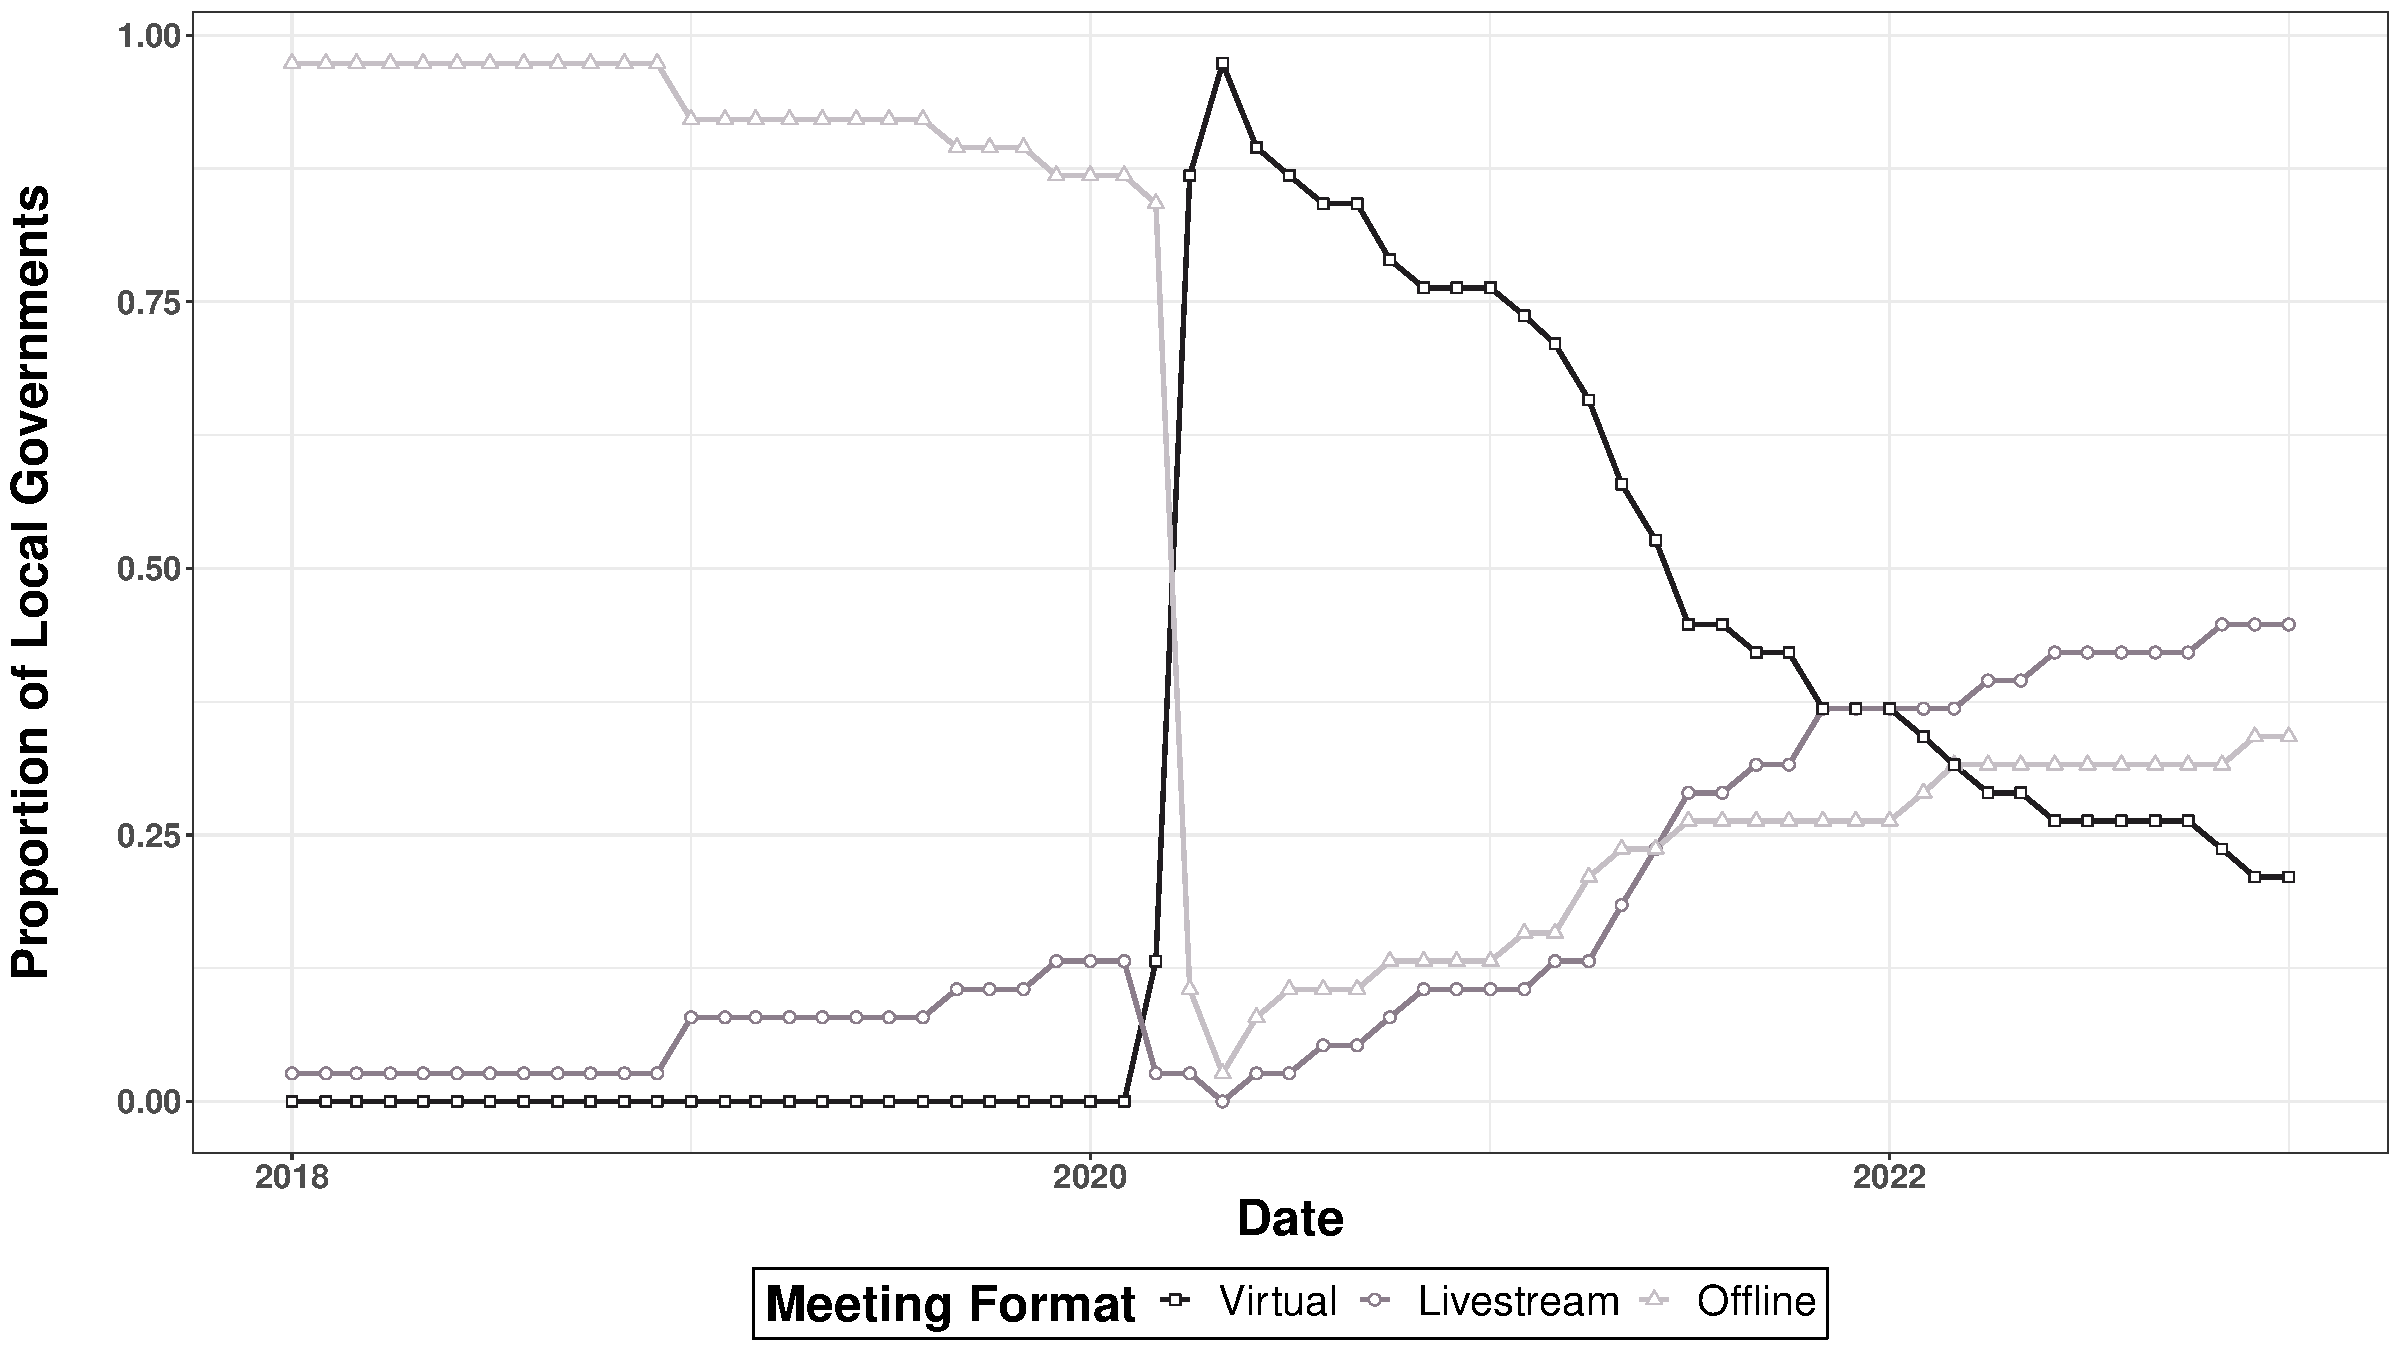
\includegraphics[scale=0.41]{Figures/OverallAccess.pdf}
        \caption[Public Meeting Formats Overtime]{The figure presents the format of local political meetings by month from January 2018 until May 2022.}
        \label{fig:OverallAccess}
    \end{figure}

    For each meeting within my dataset, I classify them into one of the three categories outlined above. As local governments conduct meetings on different schedules and cadences, I aggregate participation and access at the monthly level. I code accessibility based on whether most meetings during a given month belong to one of the three categories. \autoref{fig:OverallAccess} displays access to the local government’s meetings from 2018 until late 2022. I provide similar figures for each level of government within the Appendix. While most governments within my sample held offline meetings before the pandemic, a few cities (18\%) and school boards (6\%) experimented with holding livestreamed meetings beforehand. No governments in my sample held virtual meetings before the pandemic. Following the pandemic, however, every local government appeared to switch to some form of online meeting format. Governments then varied in terms of whether and when they switched away from online meetings, with many choosing to continue hosting online meetings in the years following the pandemic. Interestingly, livestreamed meetings became the modal meeting format for most governments, with offline meetings being the second most common. These trends, however, varied by level of government, with most cities eventually switching back to offline style meetings and both school board and county governments tending to livestreamed meetings. Virtual meetings, while the least common across all three levels of government, were still implemented by a few school board and municipal governments by the end of my sample coverage. In the following section of this paper, I leverage this staggard adoption to (and away from) online meetings to analyze whether the additional accessibility they provide translates to increased and more diverse participation.

    \section{Do Online Meetings Encourage Greater Participation?}
    \subsection{Measuring Effects on Meeting Participation:}

    In response to the developing COVID-19 pandemic, all governments within the state of Missouri were required to hold some form of online meeting from April 2020 until May 2020.\footnote{The exact order was referred to as the ```Stay Home Missouri" Order.} Following the month-long period, local governments could decide whether to switch back to offline meetings or continue hosting their meeting online. This initial shock for local governments provides near perfect opportunity to measure the impact of online meetings on public participation as I can: (1) estimate \emph{within} government effects by comparing governments before and after their switch to online and (2) estimate \emph{between} government effects by comparing governments as they adopt differing meeting formats following the pandemic. The critical question is whether the increased accessibility afforded by online meetings increased rates of public commenting. These meetings should lower the individual costs of participation and hopefully engage additional citizens. To test this initial analysis, I employ the following two-way fixed effects (TWFE) design:

    \begin{equation}\label{mod1}
        Y_{it}=\beta_0+\beta_1D_{it}+\gamma_{i}+\alpha_t+\epsilon_{it}
    \end{equation}

    \noindent where $Y_{it}$ is the total number of participants and $D_{it}$ is an indicator of whether government $i$ held primarily livestreamed, virtual, or online meetings during month $t$. The two-way government ($\gamma_i$) and month ($\alpha_t$) fixed effects to control for the time-invariant characteristics within local governments as well as monthly shocks, which may influence the number of participants at local meetings. Finally, given that I focus on the number of participants within local meetings, I model the above equation using a negative binomial regression.

    To examine whether the effects of online meetings are consistent across levels of local government, I estimate both a pooled and government-level model for each local government in my sample. I utilize the same model definition for both school board and city governments but subset the data to each respective type of government. For inference at the county level, however, my sample only includes a single county government. This fact makes it difficult to employ any form of difference-in-difference design. In order to maintain comparability and interpretability between models, I opt to employ the following simplified model:

    \begin{equation}\label{mod2}
        Y_{t}=\beta_{0}+\beta_1D_{t}+\delta_{t}+\epsilon_{t}
    \end{equation}

    \noindent where I forgo the government and month-fixed effects and substitute $\delta_t$ to capture year-based fixed effects. While this model loses the casual leverage provided by the TWFE modeling approach, it should still provide observational evidence as to whether accessibility matters for county meetings.

    \begin{figure}[H]
        \centering
         \text{The Effect of Meeting Format on Public Meeting Participation}\par\medskip
        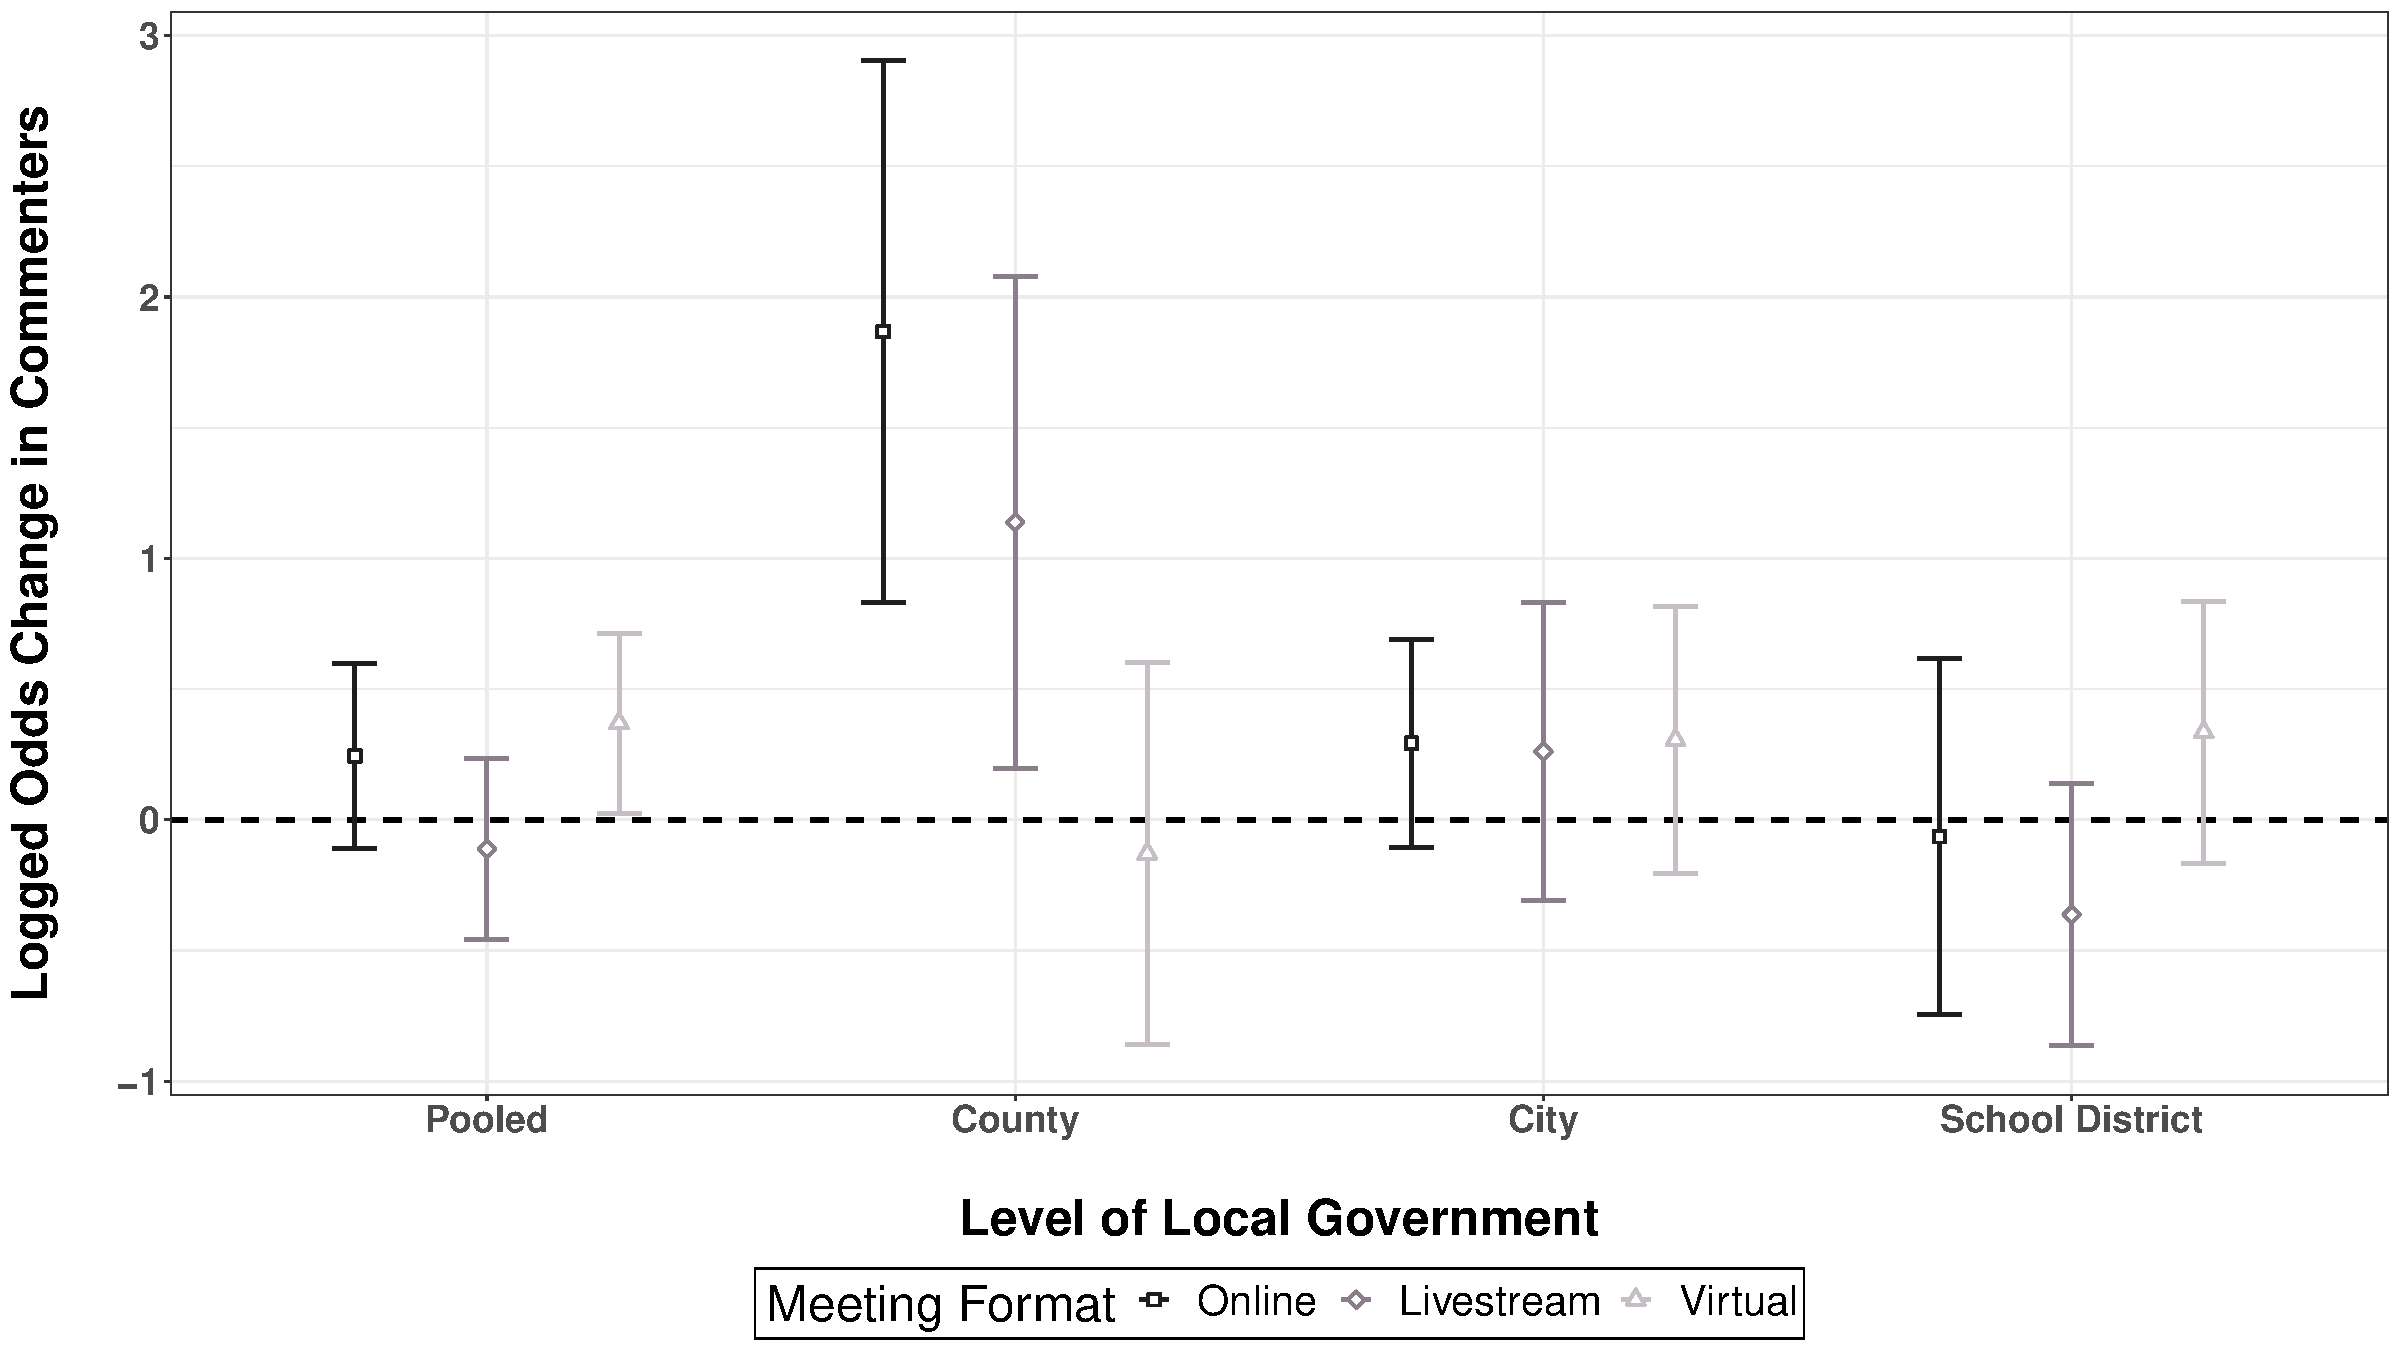
\includegraphics[scale=0.41]{Figures/MainDID.pdf}
        \caption[Effect of Meeting Format on Public Meeting Participation]{\footnotesize{Full regression results are available within the Appendix}}
        \label{fig:MainDID}
    \end{figure}

    \autoref{fig:MainDID} presents the estimated coefficients of virtual, livestreamed, and online meeting formats from my pooled and government-level models. For the pooled model, only the virtual meeting coefficient appears positive and statistically significant, with a value of 0.368. This estimate translates to a sizeable 45\% increase in the average monthly commenters or roughly 2-3 additional commenters per month.\footnote{These effects appear robust to alternative modeling strategies such as lagged dependent variable regression and the inclusion of government-level fixed effects. However, the effects lose significance but maintain direction when using more robust estimation strategies such as \citet{imaiUseTwoWayFixed2021}'s weighted linear fixed effects model.} While seemingly minor, these additional commenters could have a significant impact given the smaller scale and the increased individual political efficacy of local democracy \citep{oliverLocalElectionsPolitics2012}. Virtual meetings appear unique in their effect on meeting participation. Both online and livestreamed meetings appear not to significantly affect meeting participation. Intuitively this makes sense as virtual meetings allow individuals to participate without having to submit their comments ahead of time or physically attend. This added flexibility likely overcomes the traditional costs of meeting participation. Additionally, virtual meetings' capacity for deliberation may make participation more appealing and foster increased commenting \citep{collinsDoesMeetingStyle2021}. Interestingly, the coefficient surrounding livestreamed meetings is negative, albeit not significant. This potentially negative result could be due to livestreamed meetings' potential as a substitution rather than a promotion of meeting participation. Individuals can theoretically watch local discussions without having to participate themselves and voice their concerns only if they are not appropriately addressed within the meeting. Pooled together I find evidence that virtual meetings, in particular, fostered additional participation within local meetings, but the effect of these meetings may change between levels of local government as they vary in size and scope. 

    For the county model, livestreamed and online meetings appear to significantly increase meeting participation with coefficients of 1.139 and 1.868, respectively. Virtual meetings alone did not significantly affect meeting participation for the county. These abnormally large and significant coefficients translate to increases in meeting participants of 212\% for livestreamed meetings and 547\% for online meetings in general. Counties are geographically larger and serve more expansive constituencies; thus, they may benefit most from the added accessibility of online meetings.  Whether meeting accessibility is the sole cause of these large effects, however, is unlikely. Given the county model’s reduced form, within year time-varying confounders—namely the spread of the COVID-19 virus and discussions of racial inequities in policing—likely inflate the estimates. Examining the contents of the meeting minutes confirms this suspicion. Both meetings in which the county experienced the greatest number of participants involved discussions on reopening schools during the pandemic and the continuation of the county’s mask mandate. These meetings alone drew over 2,500 comments from citizens, far above the average 49 the county tended to receive before then. The simple fact that so many citizens \emph{could} participate may be evidence enough that accessibility matters for participation in county meetings, even if their exact causal impact is beyond the design of my simplified model.

    Turning to the city and school board models, the effects of online meetings become muddled. Online meetings of either kind do not significantly influence participation. The effect of virtual meetings is in the same direction as both the pooled and county models, but the effects of livestreamed and overall online meetings point in opposite directions for each level of government. These null effects may suggest that for these smaller governments, accessibility may matter far less than other political factors. While online meetings may remove the burden of participating in meetings, individuals may not have a reason to attend these meetings or are not engaged in local events \citep{hopkinsIncreasinglyUnitedStates2018}. Given that I find significant effects at the aggregate level, data restrictions may also be to blame as my dataset does not include enough local governments to detect the potentially nuanced effects surrounding meeting accessibility. Another possibility for the difference in effects between local government levels is that online meetings impacted some local governments and not others.

    \subsection{Did Accessibility Have Differential Effects?}
    Could online meetings affect local governments differently depending on their individual characteristics? Government and community norms may shape engagement and moderate the effects of online meetings \citep[e.g.,][]{choExperimentingPublicEngagement2021,nuamahCloseHomePlaceBased2021}. Traditional TWFE models assume homogenous treatment effects and do not allow for group-level estimates of the average treatment effect (ATE). Instead, I turn to an alternative multi-period difference-in-difference model proposed by \citet{callawayDifferenceinDifferencesMultipleTime2021}. This alternative model provides two key benefits beyond the traditional TWFE design. First, it allows for heterogenous treatment effects between groups and can estimate a separate ATE for each government in my sample.\footnote{Small groups can cause estimation problems for this model, so I follow the authors' advice and average the ATE for each group across all time periods in which they are treated.} Thus, I can estimate the effects of online meetings based on when individual (or groups of) local government(s) switch away from online meetings. Second, the model allows for the staggered adoption of treatment and therefore avoids the potential inferential concerns which can occur when applying traditional TWFE models to multi-period difference-in-difference designs \citep{imaiUseTwoWayFixed2021,sunEstimatingDynamicTreatment2021}.

    Notably, the model does require that once a unit is treated, it remains treated for the remainder of the data. Thus, I alter my previous design and leverage that all local governments had to hold some form of online meeting following the Stay Home Missouri order. In doing so, I effectively flip my treatment indicator and examine the effect of switching \emph{away} from online meetings.\footnote{No government in my sample switched back to online meetings after switching away from them.} If online meetings \emph{increase} participation, then I should find \emph{negative} treatment effects as local governments effectively lose participation by switching back to offline meetings. To leverage all possible changes in meeting accessibility, I estimate the effect of entirely switching away from online meetings and the effects of switching away from only virtual meetings. Given my focus on heterogeneous effects within local government, I estimate separate models for city and school board governments. One last assumption of the model is that units do not anticipate treatment or at least have limited anticipation of it. Local governments could theoretically anticipate switching away from online meetings and notify their constituencies, thus influencing the total number of commenters. This anticipation would bias my results and cause the estimator to become inconsistent. However, I find no evidence of anticipation when examining various lags and leads of treatment or the inclusion of various anticipation terms.

    \begin{figure}[H]
        \centering
         \text{Effect of Switching Away From Accessible Meetings By School Board Groups}\par\medskip
        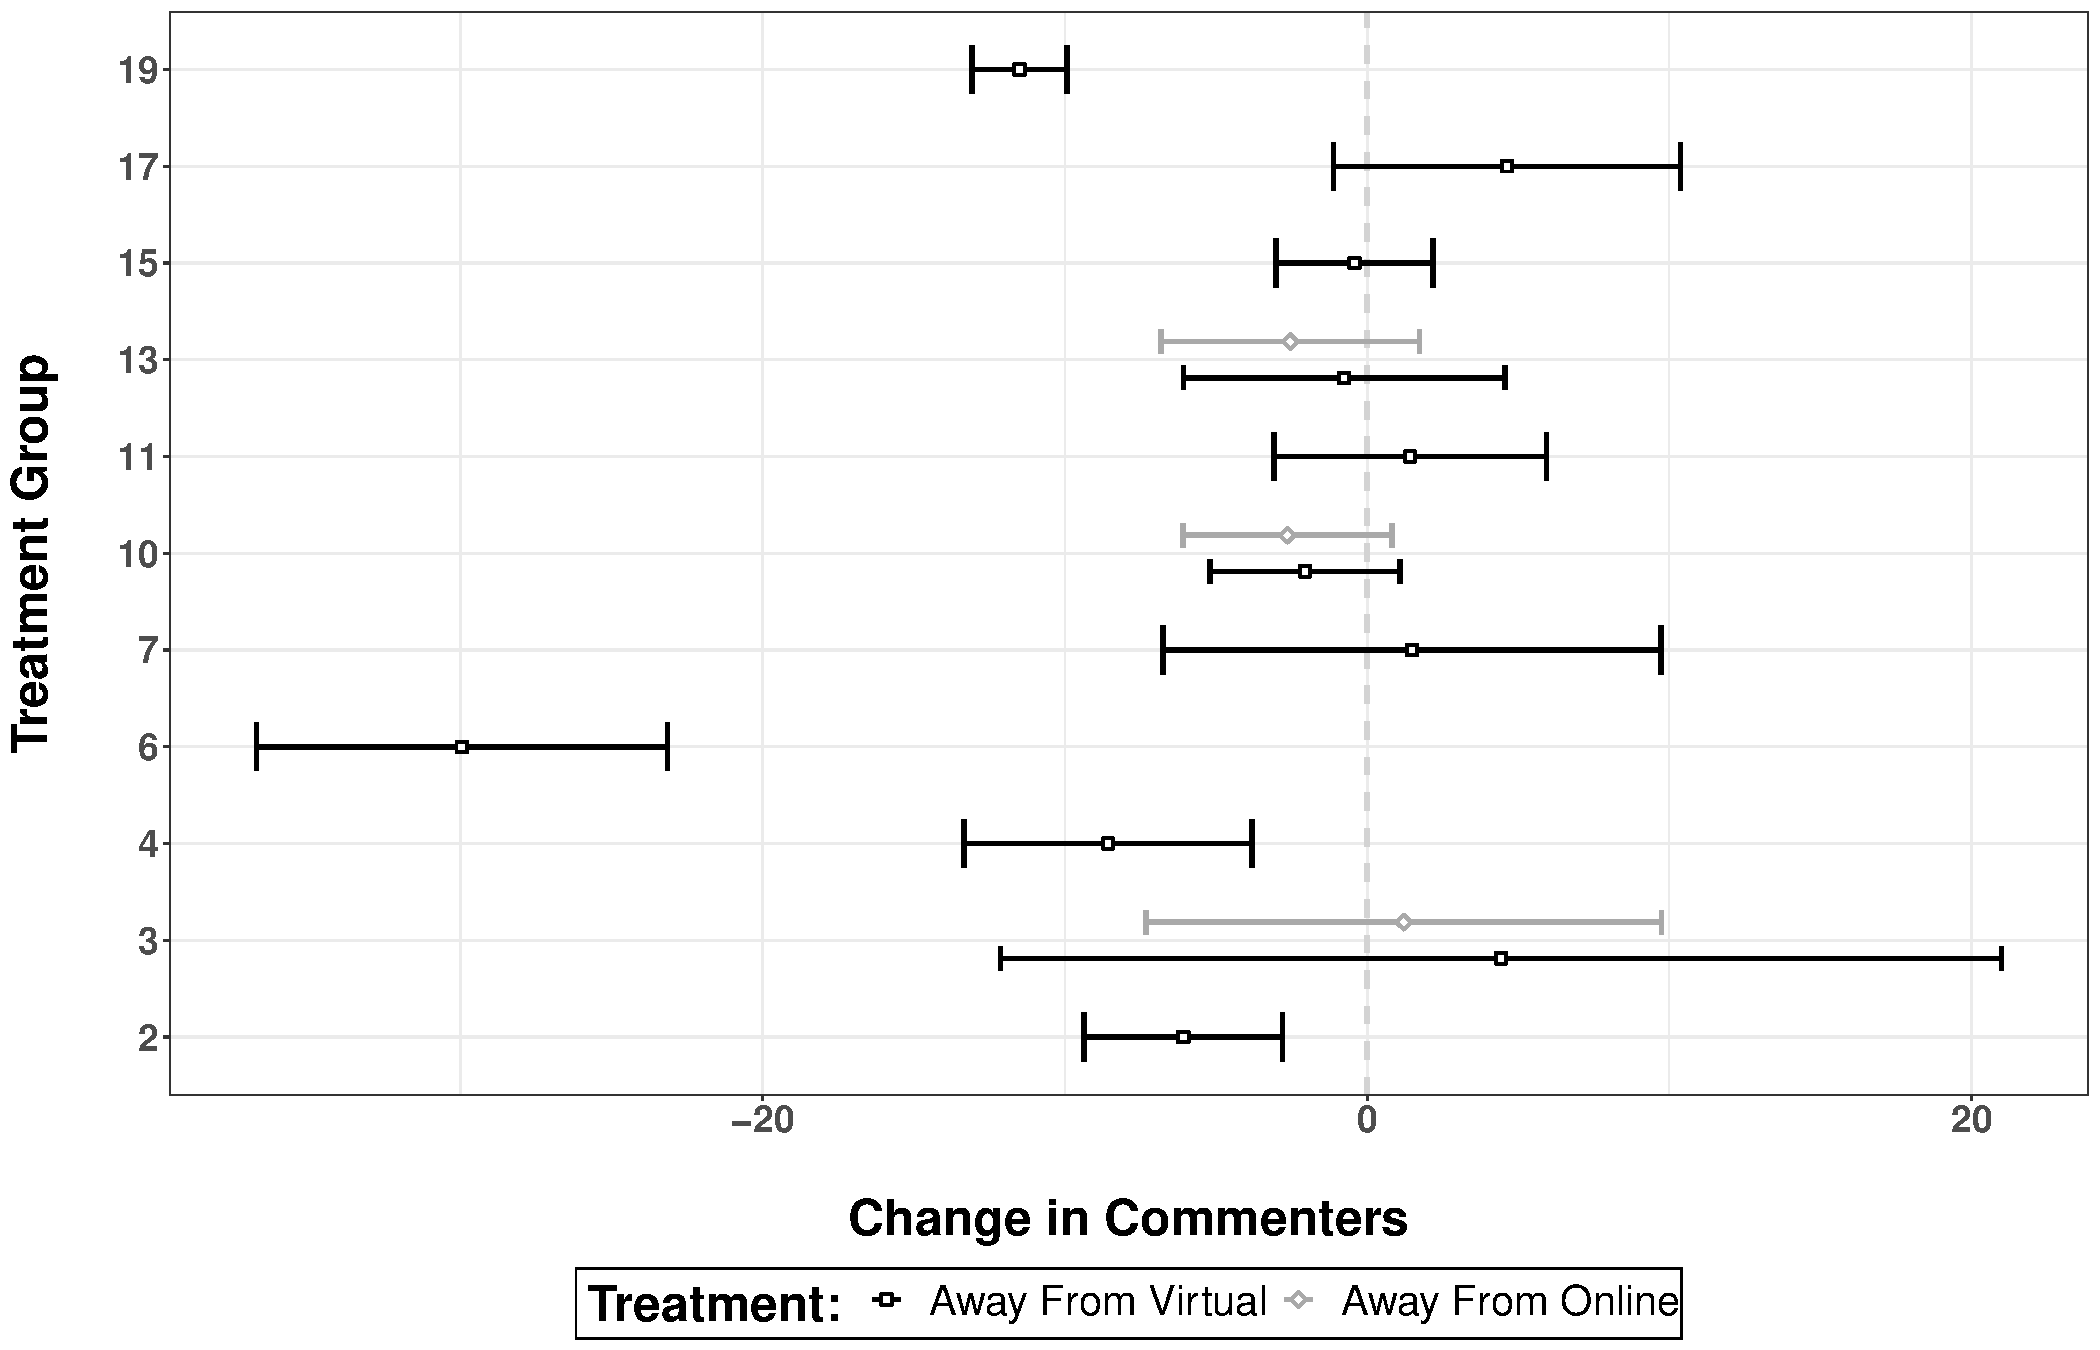
\includegraphics[scale=0.39]{Figures/SchoolMPDID.pdf}
        \caption[Effect of Switching Away From Accessible Meetings By School Board Groups]{\footnotesize{Effects are calculated using multi-period difference-in-difference design. X-axis indicates the ATE for a group averaged across all treated periods. Y-axis indicates the treatment group and the number of months passed before treatment. Standard errors are doubly robust and clustered at the group level.}}
        \label{fig:AwaySchool}
    \end{figure}

    \autoref{fig:AwaySchool} and \autoref{fig:AwayCity} present the differential effects of switching away from online meetings for cities and school boards within my sample. The y-axis indicates the treatment group and the number of months before it was treated. For example, group two in \autoref{fig:AwaySchool} switched away from virtual meetings two months after the Stay Home Missouri order started. Across both models, all but two groups consisted of a single government. The x-axis captures the group specific ATE in the change of monthly commenters. Immediately apparent, virtual meetings appeared to have differential effects within and between school boards and city governments. Most school boards saw no change in their number of monthly commenters. However, three experienced significant losses in meeting participation after switching away from virtual meetings, with one school board experiencing an estimated decline of 29 monthly commenters. The opposite appears true for cities. Most cities similarly experienced no change in their average monthly commenters; however, in the case of two cities, switching away from online meetings had a positive and significant effect on meeting participation. For these cities, switching away from online meetings increased their monthly commenters by roughly a single additional commenter.

    \begin{figure}[H]
        \centering
         \text{Effect of Switching Away From Accessible Meetings By City Groups}\par\medskip
        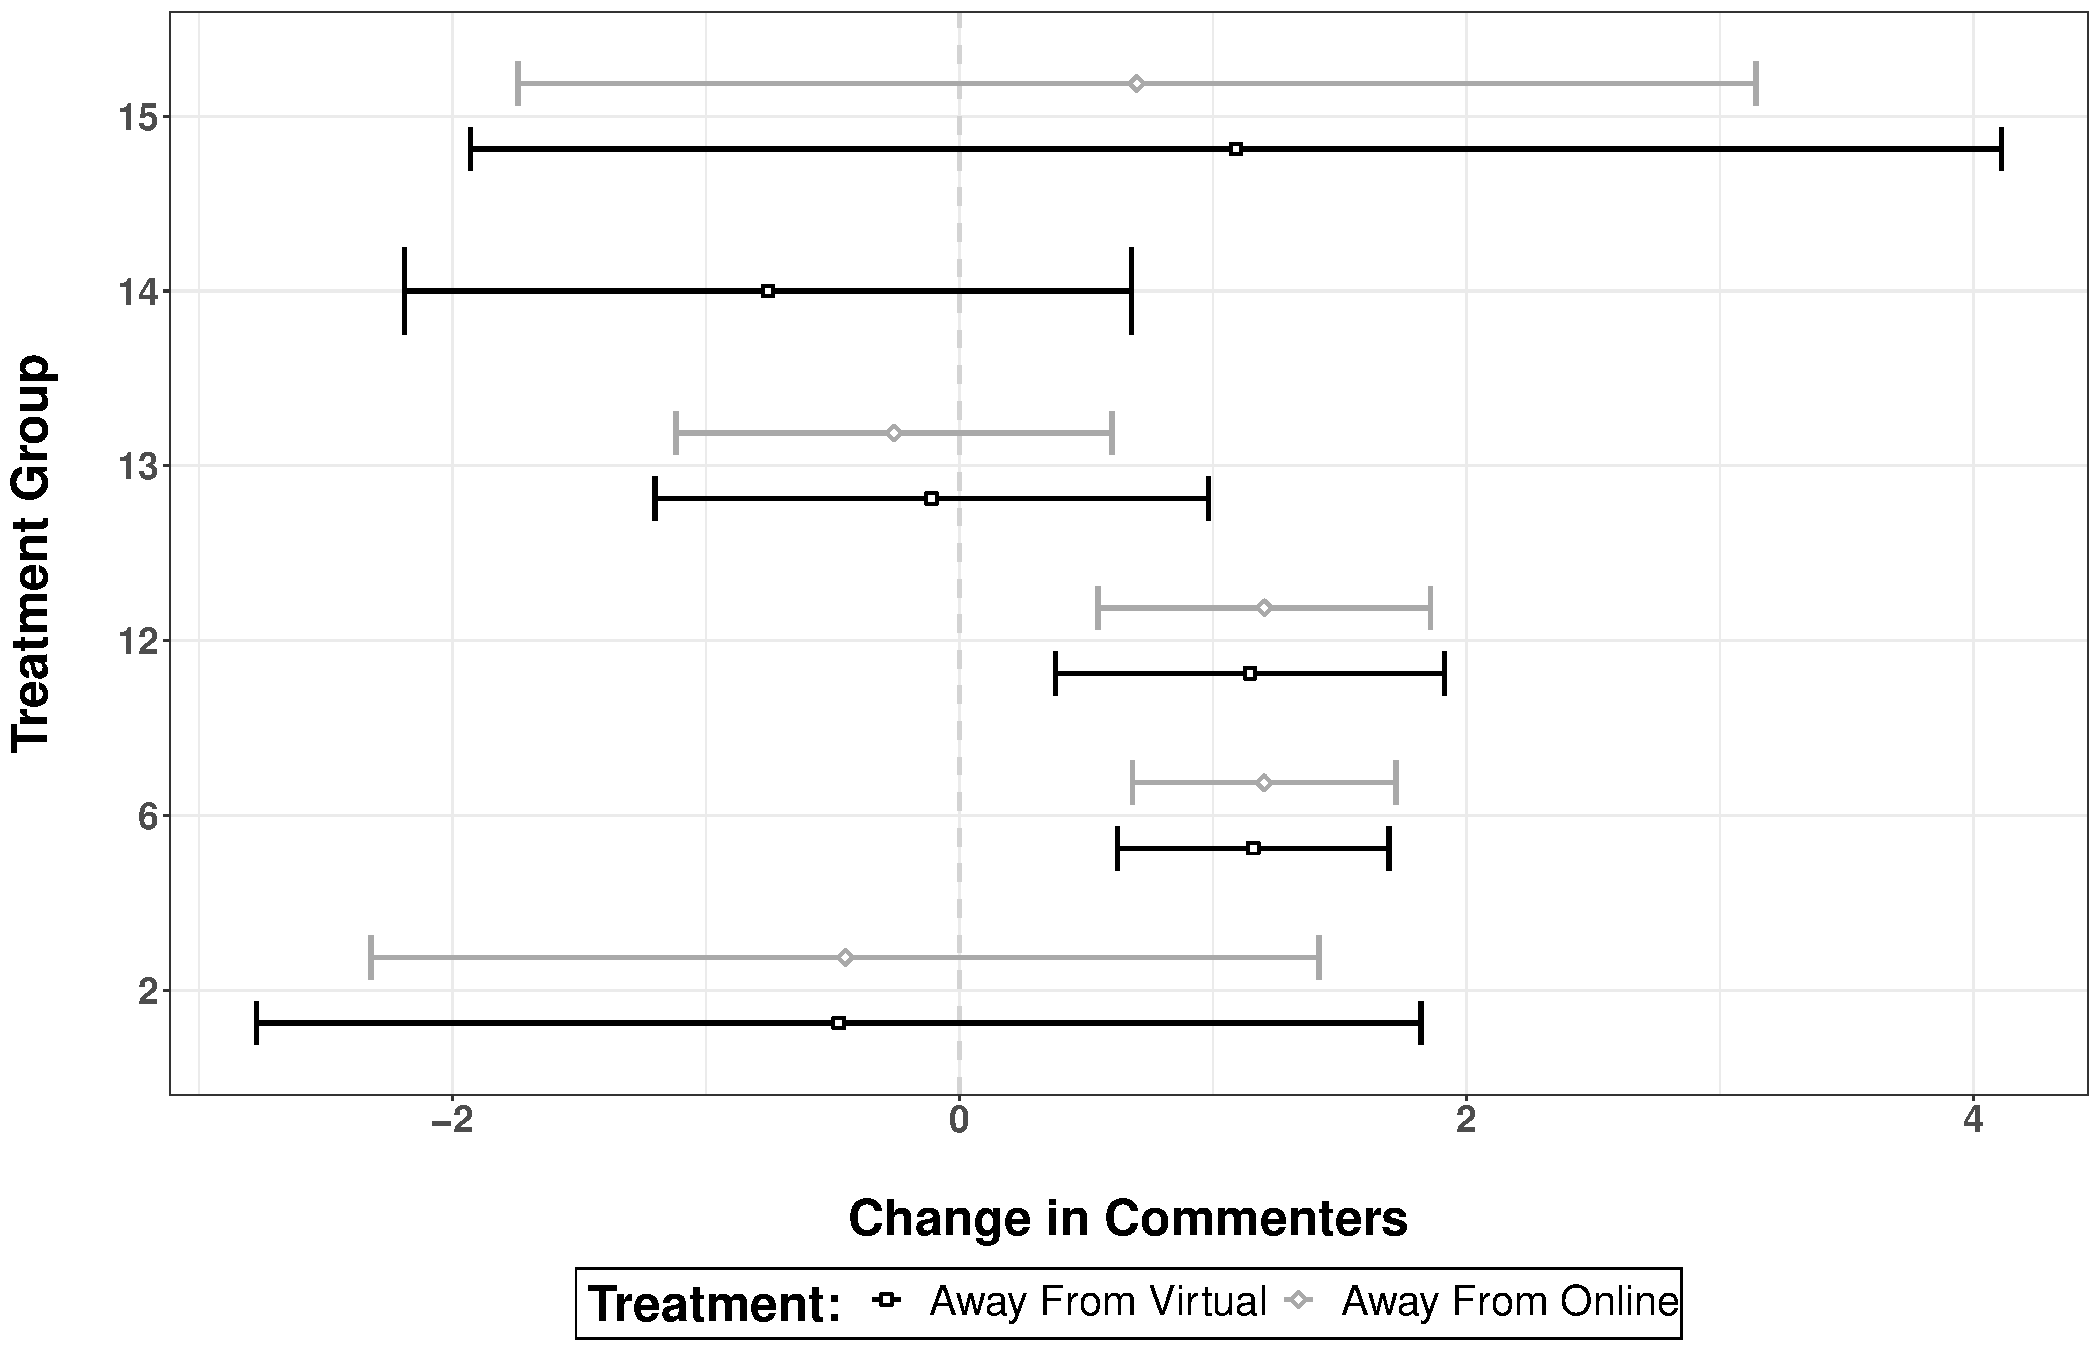
\includegraphics[scale=0.39]{Figures/CityMPDID.pdf}
        \caption[Effect of Switching Away From Accessible Meetings By City Groups]{\footnotesize{Effects are calculated using multi-period difference-in-difference design. X-axis indicates the ATE for a group averaged across all treated periods. Y-axis indicates the treatment group and the number of months passed before treatment. Standard errors are doubly robust and clustered at the group level.}}
        \label{fig:AwayCity}
    \end{figure}

    Beyond group-level estimates of the effect of online meetings, these models can also provide additional insight regarding the effect on cities and school boards as a whole. Following \citet{callawayDifferenceinDifferencesMultipleTime2021}, I average the group-level effects to obtain overall estimates of the ATE. Doing so provides a significant effect of -4.30 for school boards switching away from virtual meetings and a non-significant effect of -1.3 for switching away from online meetings altogether. For cities, both the effect of switching away from virtual meetings (0.324) and online meetings (0.32) appear positive but not significant. While the effect of virtual meetings contrasts those found within the school specific TWFE model, it is similar in size to the estimated effects found within the pooled model. 
    
    Since I group governments by treatment timing, I also can examine how said timing may influence the effects of online meetings. Theoretically, how quickly a government switches away from online meetings may moderate their experience as citizens and public officials have varying amounts of time to become familiar with the new meeting styles. In the case of both school boards and cities, I find some evidence that those governments who switch sooner experience more significant changes, but the effect appears to be inconsistent. Not accounting for those with null effects, school boards who switched away from virtual meetings 2-4 months after the Stay Home Missouri order experienced roughly the same participation loss as those who switched a year later. No apparent pattern exists for cities changing away from virtual or all online meetings. These findings suggest that the effects of online meetings are likely more centered on individual government characteristics rather than the timing of their choice to switch.

    Overall, this evidence, combined with that of my primary models, suggests that meeting accessibility positively affected participation within local democracy. However, this boost was inconsistent across and within levels of local government. Some governments experienced a drastic increase in participants, while others experienced no change or a slight decline. Given this potential for increased participation, it is essential to understand whether accessibility brings diverse voices or further instills pre-existing inequities in local participation.

\section{Do Online Meetings Lead to More Diverse Participants?}

\subsection{Obtaining Commenter Characteristics:}
In the previous section, I found that more accessible meetings can foster increased participation, albeit the effect varies across local contexts. Are these meetings bringing new voices to local meetings or instilling previous inequities in participation? To answer this question, I match each commenter in my dataset to a commercial voter file provided by L2. This file contains both previous records of political activity and demographic estimates for each individual. I utilize the \texttt{fastLink} package in R to probabilistically match commenters on first name, last name, and address \citep{enamoradoUsingProbabilisticModel2019}. While probabilistically matching commenters can lead to higher rates of false positive matchings in which I incorrectly match commenters to voters, it decreases rates of false negatives and increases my overall match rate. The process also allows me to include measures of matching uncertainty within my later analyses. Given the voter file holds more than 650,000 records for the St. Louis region alone, I block voters first on government boundaries and then on zip code.\footnote{When matching county commenters, I only block voters based on zip code} This process aims to narrow down the universe of possible matches and improve matching rates. I follow previous work matching commenters to administrative records and match commenters with a match threshold of 0.85 \citep{yoderDoesPropertyOwnership2020}. In other words, two records are considered a match if the posterior probability of said match is greater than 85\%. Before examining whether online meetings encouraged diverse meeting participation, my sample provides a novel opportunity to characterize commenters across local contexts.


\subsection{Characterizing Commenters Across Local Contexts}
\autoref{fig:CommentDemo} displays the difference in means between commenters and all voters living within the region. For this initial analysis, I pool commenters across all meeting formats. Regarding school boards and cities, I subset to only voters residing within the jurisdiction of my sample. To account for the uncertainty in my matching procedure, I down-weight each estimate by my match threshold (0.85) as prescribed by \citet{enamoradoUsingProbabilisticModel2019}. Previous studies of commenting within municipal politics find that individuals who comment are whiter, weather, older, and more likely to be homeowners than their immediate communities \citep{einsteinWhoParticipatesLocal2019,yoderDoesPropertyOwnership2020}. I find broadly consistent findings when examining cities in my sample. City commenters stand out as predominantly whiter and older, with a higher likelihood of being homeowners and actively participating in national and local elections. Interestingly, I do not find a significant overrepresentation of men as consistently documented in previous studies \citep[e.g,][]{einsteinStillMutedLimited2022}, albeit the coefficient is in the same direction.

\begin{figure}[H]
    \centering
     \text{Difference Between Voters and Commenters}\par\medskip
    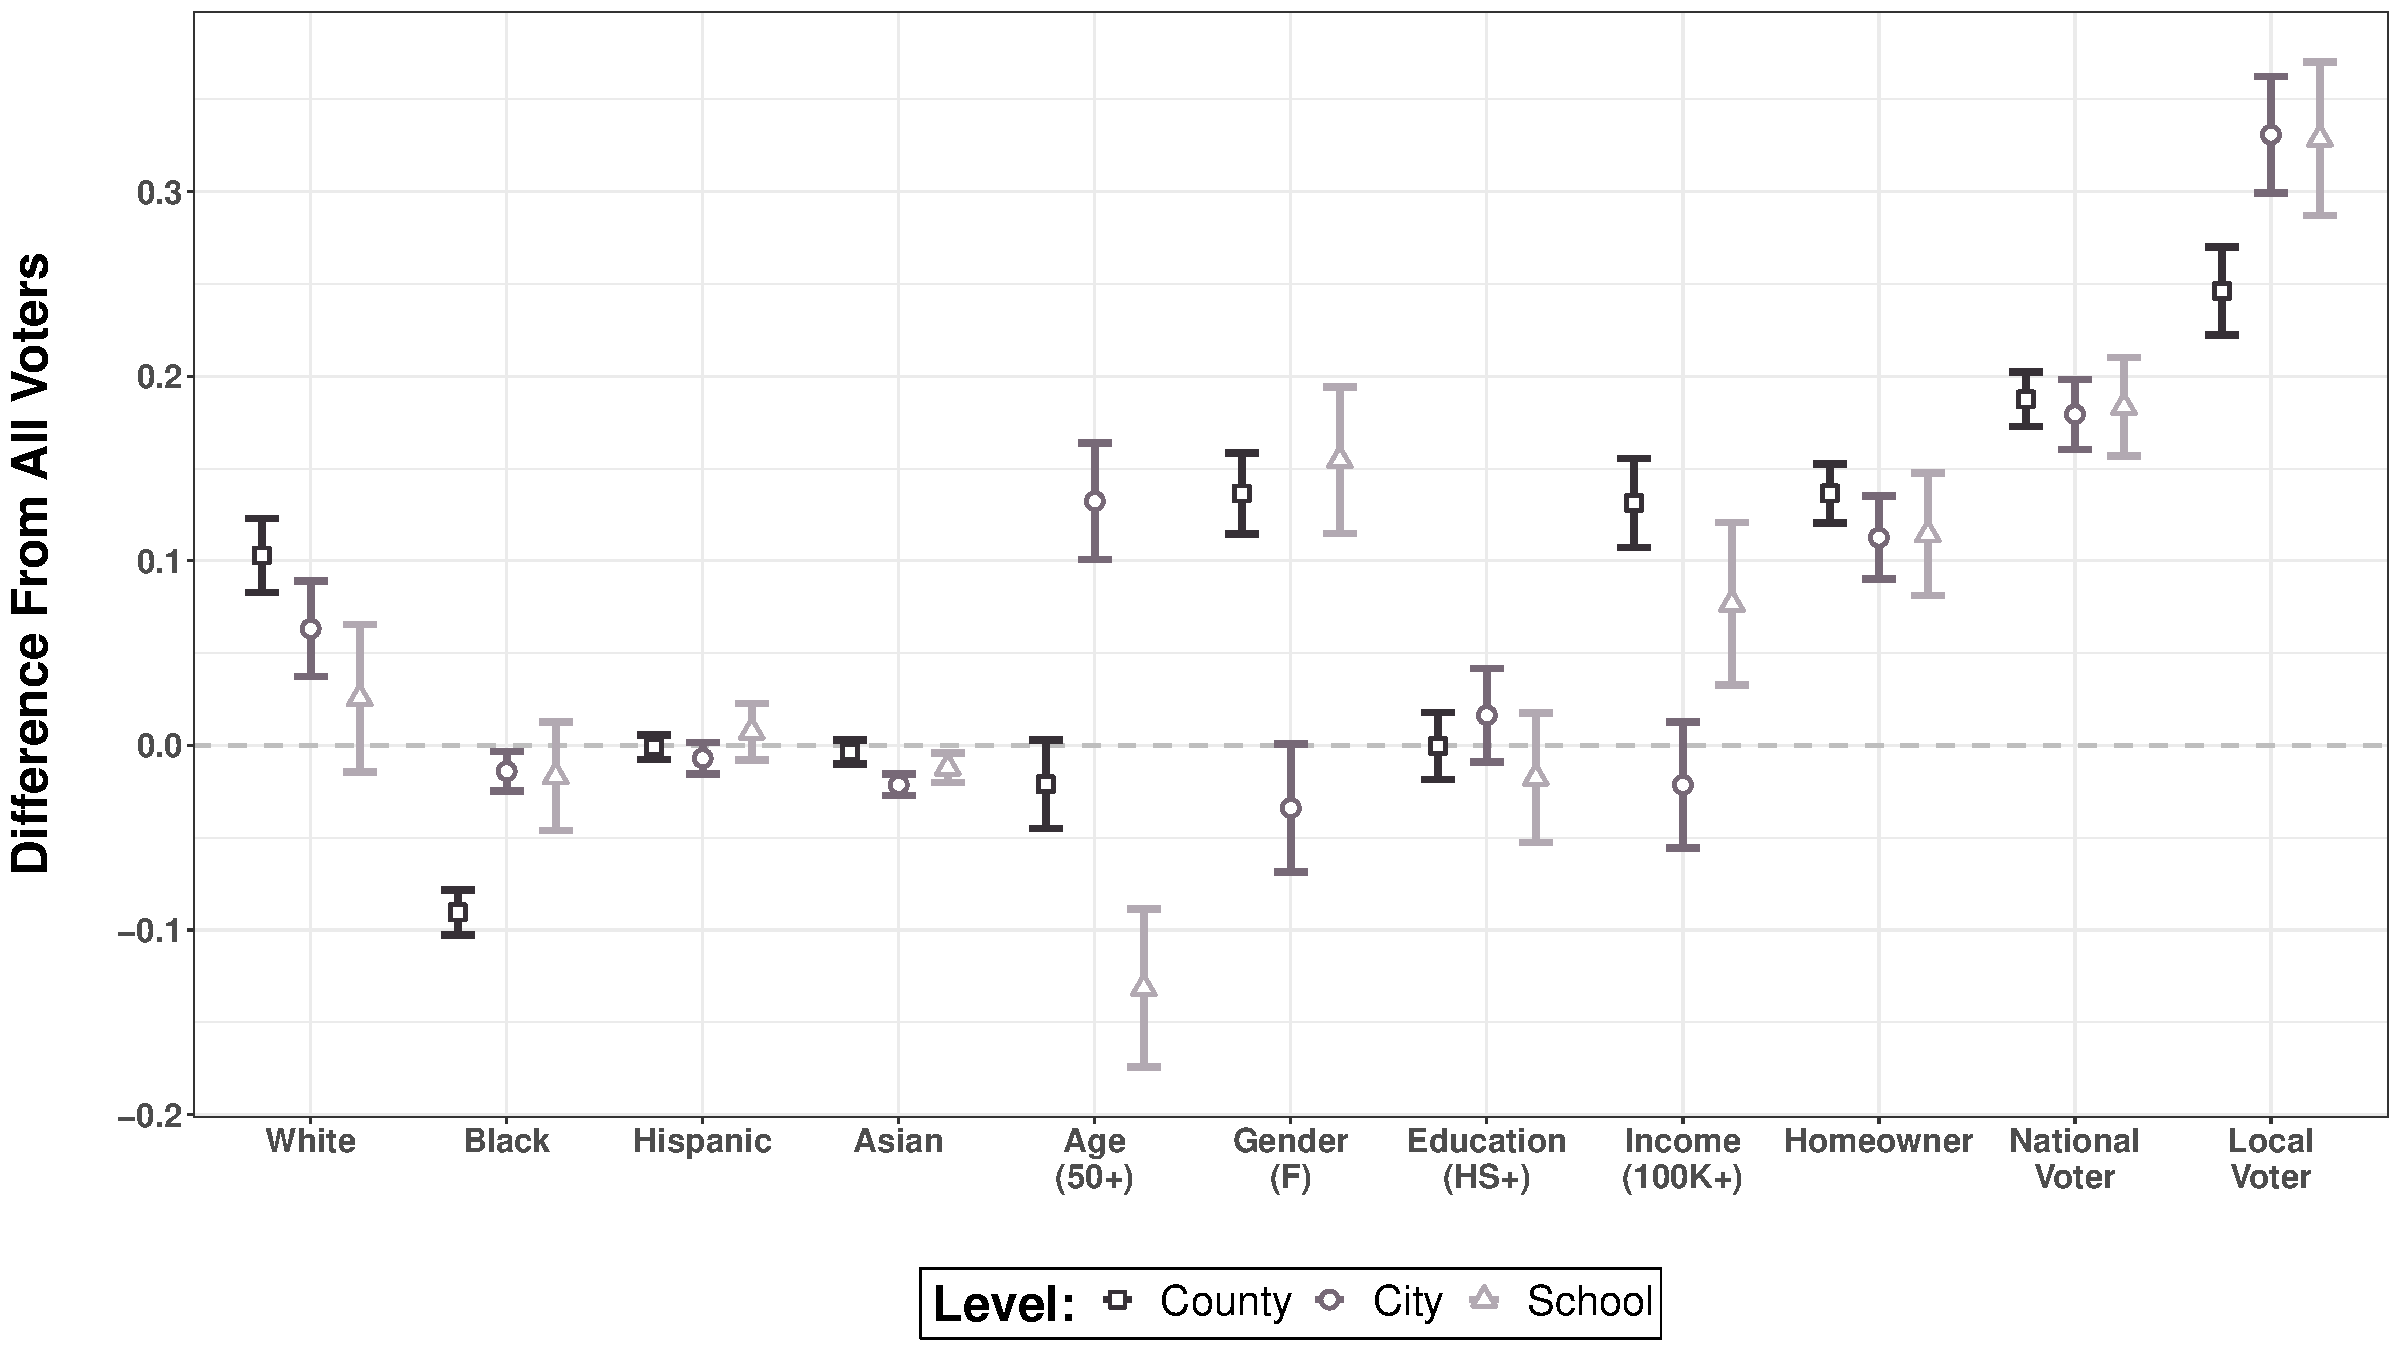
\includegraphics[scale=0.41]{Figures/CommentDemoPooled.pdf}
    \caption[Difference Between Voters and Commenters]{\footnotesize{Commenters are pooled across all meeting formats. School and city comparisons are subset to their repective voters. Simultaneous comparisons are available in the Appendix.}}
    \label{fig:CommentDemo}
\end{figure}

County governments deal with inherently different issues and represent larger constituencies; however, they are still comparable to local governments in terms of services and powers. When examining the differences between county commenters and their surrounding communities, I find that they also suffer from similar participation inequities as in municipal politics, albeit with several key differences. Commenters are similarly whiter and wealthier, with a higher likelihood of being homeowners and politically active but are not so different from their communities regarding education or age. One of the most surprising differences is that significantly more women comment at the county level. These effects may be due to counties handling issues related to health and welfare, two policy areas women lawmakers are more likely to prioritize \citep[e.g., ][]{huddyConsequencesGenderStereotypes1993, voldenWomenIssuesTheir2018, paysonDecomposingSourceGender2023}. Additionally, the pandemic's gender-specific impacts may have motivated women to participate at greater rates \citep{carrerasWhoDoesCaring2023,johnsonGenderPoliticalLeadership2020}. I find similarly high rates of women participating in school board meetings.

Commenters at school board meetings are younger and more likely to be women than their surrounding communities. Intuitively this makes sense, given the traditional and gendered role women tend to hold within households, and younger individuals are more likely to have school-age children. Thus, these two groups are more likely to have a vested interest in school board outcomes. These gendered effects, in particular, provide a new perspective on the difference in gendered political participation within local politics \citep{coffeSameGameDifferent2010}. Importantly they highlight yet another dimension along which the pandemic potentially impacted genders differently. Along other demographics, school commenters appear to vary from their communities in unique ways. While commenters are more likely to be wealthier, own homes, and vote in recent elections, they do not differ significantly in terms of race. Surprisingly, school board commenters largely resemble the racial makeup of their surrounding communities. This lack of difference may be partly due to the well-documented mobilization of minority communities to protect school resources \citep{morelTakeoverRaceEducation2018,nuamahCloseHomePlaceBased2021,kitchensExitInvestSegregation2021}. However, this seemingly equal participation in public meetings may come at an increased cost of participation paid on behalf of Black individuals especially \citep[see][]{nuamahCostParticipatingPoor2021}. Overall, school board, county, and city commenters appear significantly different from their surrounding communities but do so uniquely depending on the local context and policy priority of the local government.


\subsection{Measuring the Difference Between Online and Offline Commenters}

Online meetings should, in theory, lessen the burdens of political participation faced by different groups and potentially increase the diversity of commenters. However, previous work examining online meetings in the context of planning and zoning meetings has found them to largely attract the same demographics and fail to address inequities in meeting participation \citep{einsteinStillMutedLimited2022}. To examine the effects of online meetings across my sample, I calculate the difference in means between online and offline commenters relative to all voters living within my sample’s geographic coverage. Doing so allows me to compare commenters to those from alternative meeting formats as well as their communities. \autoref{fig:OnOffDemo} displays the difference means between each group, again adjusted by my match uncertainty.

\begin{figure}[H]
    \centering
     \text{Difference Between Voters and Commenters By Meeting Format}\par\medskip
    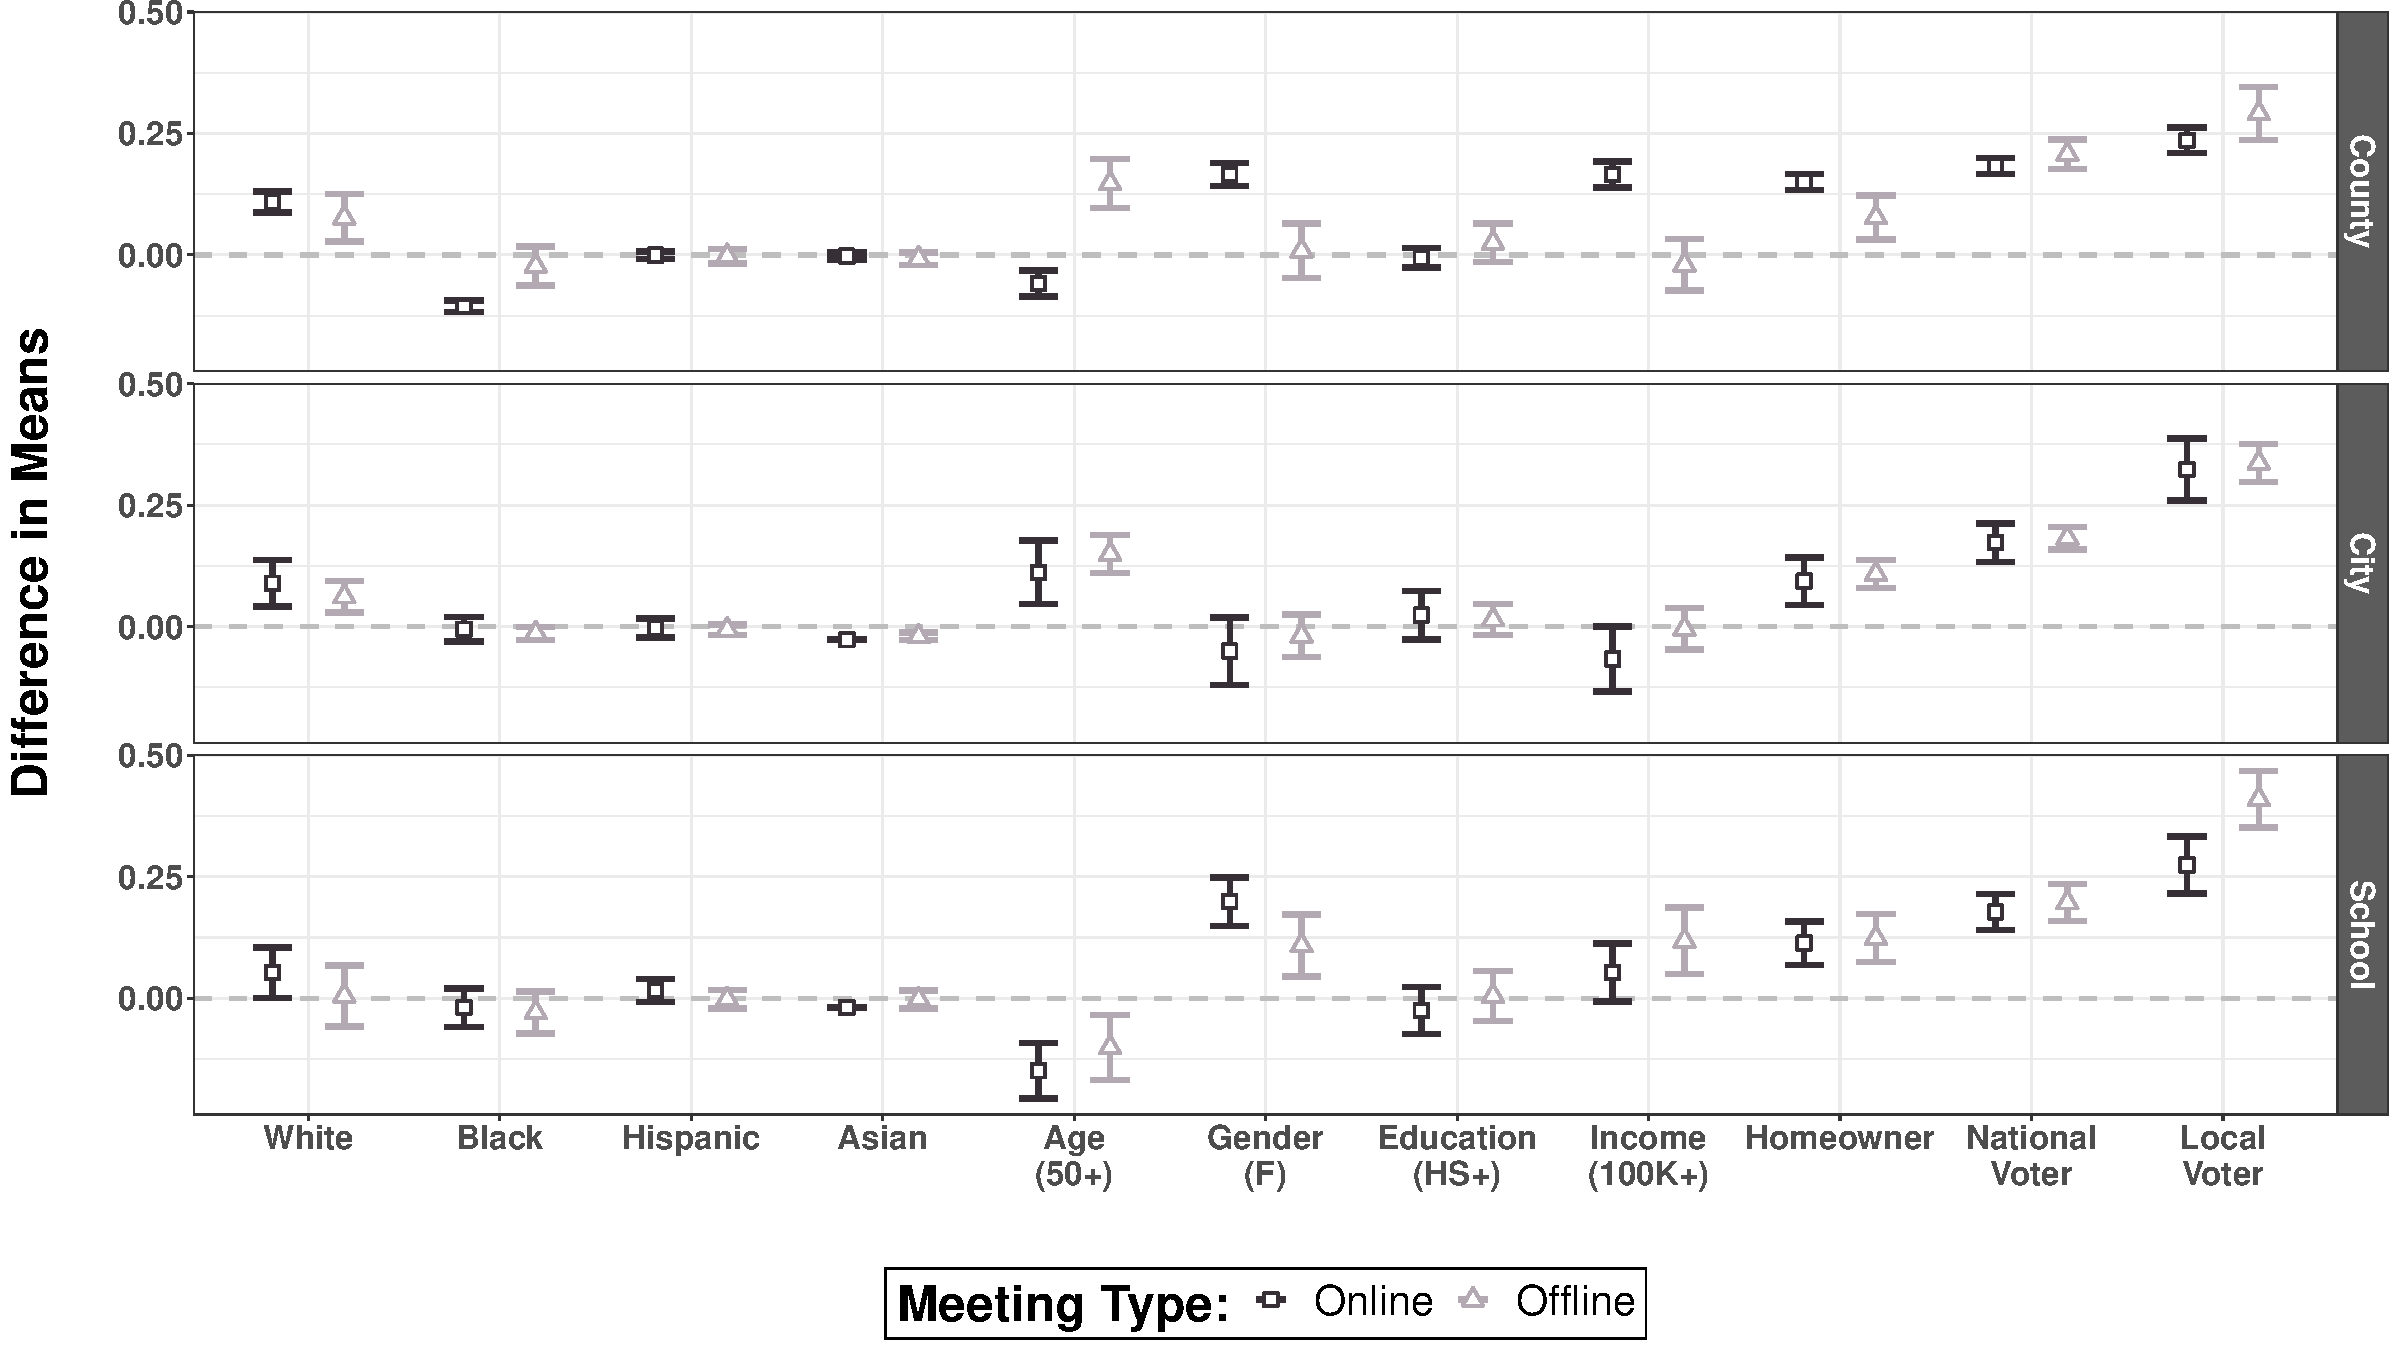
\includegraphics[scale=0.45]{Figures/OnOffDemoComparison.pdf}
    \caption[Difference Between Voters and Commenters By Meeting Format]{\footnotesize{School and city comparisons are subset to their repective  voters. Estimates are adjusted to account for uncertainty in the matching process. Simultaneous comparisons are available in the Appendix.}}
    \label{fig:OnOffDemo}
\end{figure}

Overall, online commenters across all three local contexts are similar to their offline counterparts. They tend to be misrepresentative of their communities along dimensions of race, income, and political engagement. For the county, online meetings did attract significantly more women and younger commenters. Online meetings, in particular, appear responsible for the over-representation of women identified in my pooled analysis above. However, these benefits came at the cost of widened gaps in racial representation, income, and homeownership. In the case of cities, I document no noticeable change between online and offline commenters, with results similar to \citet{einsteinStillMutedLimited2022} examination of online meetings. Finally, for school boards, online meetings attracted more individuals previously not engaged in local elections and potentially lessened the divide in income, albeit the estimate is not statistically distinguishable from that of offline commenters. Beyond these characteristics, I find no substantial differences between online and offline school board commenters.

Despite the theoretical benefits of online meetings, I find they had a mixed effect on the diversity of meeting participants. For the county and school boards in my sample, online meetings lessened some divides and incentivized an over-representation of traditionally underrepresented groups; however, many previous inequities in participation persisted within these meetings. Online meetings appeared even to exacerbate some disparities in the county's case. Notably, my approach above does not account for time or geographic varying confounders, which may alter specific demographics' propensity to comment. To partially address this concern, I utilize a logistic regression to examine differences between online and offline commenters simultaneously with added geographic controls. I present the results within the Appendix and find substantively similar results.

\section{Discussion:}
Online meetings were adopted out of necessity in response to the pandemic but offered a potential solution to historically low engagement in local political meetings. These meetings act as a crux for local democracy and allow individuals a direct connection to local public officials and policy-making processes. Given historic inequities in who attends and the resulting policy outcomes, increasing the quantity and diversity of meeting participants is vital to the healthy functioning of local democracy. Utilizing a novel dataset of meeting commenters, I find that online meetings are an effective tool to expand access to local governments, but in isolation, they are insufficient to address pre-existing inequities in who participates within local democracy. What’s more, I find that inequities in participation previously found within municipal politics are present within both county and school board contexts. However, I find some silver lining for local democracy as some groups—namely women—appear to be overrepresented within some levels of local politics. This finding suggests that some groups may effectively make up for underrepresentation in local politics by being overly active in other potentially more relevant local contexts. Future work should explore whether these potential increases in participation manifest into meaningful policy change for these often-underrepresented groups.

For policymakers, these results bring mixed news. On one hand, accessibility matters for local government and can boost the number of voices heard within local meetings. What’s more these voices at least appear to be sincere. Section A.4 of Appendix I shows evidence that online participants share jurisdictionally relevant comments and, contrary to fears of trolling or increased incivility, do so with a similarly positive sentiment as their offline counterparts. However, improving access is no panacea for the deep-rooted inequities present within local politics. In fact, improving accessibility, when implemented alone, may do more harm than good by exacerbating existing inequities in political participation. To truly address these problems, policymakers likely need to find a way to empower individuals and their communities and improve their sense of political efficacy. If individuals do not believe their voice can impact local policy outcomes, allowing them to attend virtually will likely not persuade them to participate. 
